\documentclass{llncs}
%
%
%espero que no se enfaden por incluir este paquete:
\usepackage{amsmath}
\usepackage[dvips]{graphicx}
\usepackage{makeidx}  % allows for indexgeneration

\hyphenation{pro-per-ties}
\hyphenation{ge-ne-ral-ly}
\hyphenation{pre-fe-ren-ces}
\hyphenation{u-sing}
\hyphenation{pu-nish-ment}

\begin{document}

\mainmatter              % start of the contributions
%
\title{On the cartesian product and the join operations in temporal databases}
%\title{Introducing valid time in bipolar database querying}
%
%\titlerunning{A Fuzzy Valid-Time Model}  % abbreviated title (for running head)
%                                     also used for the TOC unless
%                                     \toctitle is used
%
\author{\and Jose Enrique Pons\inst{1} \and Christophe Billiet\inst{2} \and Guy De Tr\'e\inst{2} \and Olga Pons Capote\inst{1} }

%
%\authorrunning{Ivar Ekeland et al.} % abbreviated author list (for running head)
%
%%%% list of authors for the TOC (use if author list has to be modified)
%\tocauthor{Ivar Ekeland, Roger Temam, Jeffrey Dean, David Grove,
%Craig Chambers, Kim B. Bruce, and Elisa Bertino}
%
\institute{Department of Computer Science and Artificial Intelligence \\
University of Granada \\
C/Periodista Daniel Saucedo Aranda s/n E-18071 (Granada-Spain) \\
\email{jpons,opc@decsai.ugr.es}\\ 
%WWW home page:
%\texttt{http://users/\homedir iekeland/web/welcome.html}
%\and
%Universit\'{e} de Paris-Sud,
%Laboratoire d'Analyse Num\'{e}rique, B\^{a}timent 425,\\
%F-91405 Orsay Cedex, France
\and 
Department of Telecommunications and Information Processing,\\
Ghent University,\\
Sint-Pietersnieuwstraat 41, B-9000 Ghent, Belgium\\
\email{Christophe.Billiet,Guy.DeTre@UGent.be}
}

\maketitle              % typeset the title of the contribution

\begin{abstract}

%%%%%%%%%%%%%%%%%%%%%%%%%
%
% ABSTRACT
%
%%%%%%%%%%%%%%%%%%%%%%%%
In reality, some objects or concepts have properties with a time-variant or time-related nature. Modelling these kinds of objects or concepts in a (relational) database schema is possible, but time-variant and time-related attributes have an impact on the consistency of the entire database. Therefore, temporal database models have been proposed to deal with this. Time itself can be at the source of imprecision, vagueness and uncertainty, since existing time measuring devices are inherently imperfect. Accordingly, human beings manage time using temporal indications and temporal notions, which may contain imprecision, vagueness and uncertainty. However, the imperfection in human-used temporal indications is supported by human interpretation, whereas information systems need support for this. Several proposals for dealing with such imperfections when modelling temporal aspects exist. Some of these proposals transform the temporal expression into a compact representation. Other proposals consider the temporal indications in the used temporal expressions to be the source of imperfection. 
In this work we present a novel model to deal with imperfections in valid-time databases. Next to that, the data manipulation language, \emph{DML} is defined and implemented.

\end{abstract}

%
\section{Introduction}

%
%Information systems (IS) have always tried to model parts of reality. To achieve this modelling, such systems contain data representing properties of real-world objects or concepts~\cite{JoseEnriquePons2012},~\cite{Billiet2012}. As time is an essential aspect of many real-world objects or concepts, information systems often contain data representing temporal notions which describe such temporal properties~\cite{Bolour1982},~\cite{VanderCruyssen1997}. Such temporal notions usually take the form of either instants~\cite{Jensen1998}, which can informally be seen as infinitely short `moments' or `points' in time, or time intervals~\cite{Jensen1998}.

Data are often produced by humans, but human-made data are prone to imperfections: some data may be vague, imprecise, incomplete, contradictory or uncertain. Data representing temporal notions may contain such imprecisions too~\cite{Devos1994},~\cite{Dubois2003},~\cite{JoseEnriquePons2012},~\cite{Billiet2012}. The work presented in this paper is specifically concerned with time intervals (and as a special case: instants) subject to uncertainty.

Generally, one of the most important purposes of an IS is to allow the retrieval of information or knowledge deduced from its data. Information or knowledge is usually retrieved from an IS by querying it and examining or analyzing the query results or by visualizing the contents of the IS, querying this visualization and examining or analyzing the resulting visualization(s).

Of course, when temporal information is represented in an IS, querying this IS may have a temporal aspect too. Usually, querying an IS containing data representing temporal notions is conceptually done by specifying one or more time indications and requesting information that is in a specific relationship with these indications, where the semantics of these relationships are specifically temporal~\cite{Billiet2012},~\cite{JoseEnriquePons2012},~\cite{Pons2012a}. Thus, some existing proposals have considered groups of basic relationships between time indications used to construct and express specific temporal relationships~\cite{Medina1994},~\cite{Schockaert2008}. Notably, Allen~\cite{Allen1983} presented a reasoning framework containing all semantically usefull basic temporal relationships between time intervals (and as a special case instants). The resulting relationships are shown in figure \ref{fig:allen-relationships}. These Allen relationships are used in the presented work.

\begin{figure}[h]
   \centering
   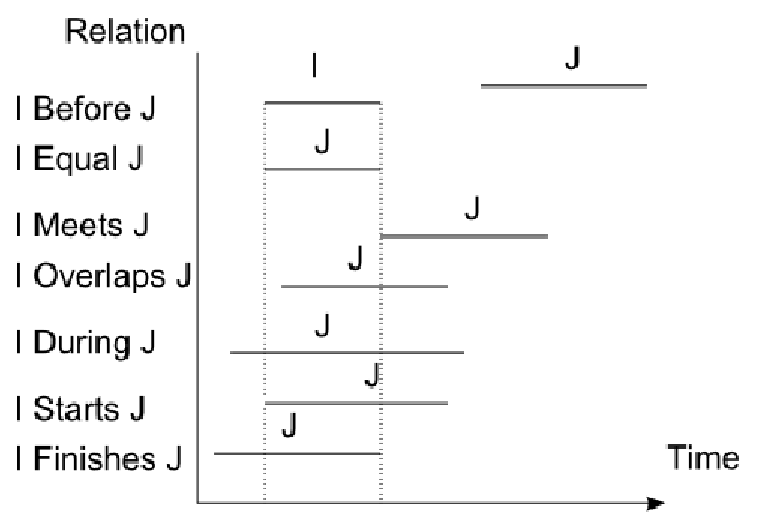
\includegraphics[width=0.9\columnwidth]{graphs/allen.eps}
   \caption{The Allen relationships between two crisp intervals $I$ and $J$.  }
   \label{fig:allen-relationships}
 \end{figure}

To be able to query IS containing data representing time indications subject to uncertainty, a framework is necessary, able to represent uncertainties in time indications in a semantically sound way, without (much) information loss and able to temporally reason with such time indications in a semantically sound and usefull way~\cite{Dubois1983},~\cite{Dubois2003}. Although more proposals for such frameworks exist, the work presented in this paper focusses on just two: the \emph{ill-known constraint \emph{(IKC)} framework}~\cite{Pons2011} and the \emph{triangular model \emph{(TM)} framework}~\cite{DeTre2012}.

The work presented in this paper consists of a comparison of both frameworks, about the approaches they use to represent time intervals subject to uncertainty and to reason about the temporal relationships between such intervals and time intervals without uncertainty.

The structure of this paper is as follows: section \ref{sec:general-preliminaries} presents some general preliminaries and naming and notation conventions used in this paper. Sections \ref{sec:ikc} and \ref{sec:tm} introduce the IKC and TM frameworks respectively: both sections first introduce some preliminary concepts and techniques specific to the framework under consideration, then explain how the representation of time intervals by the framework is done and finally show how the evaluation of Allen relationships between an interval subject to uncertainty and one without uncertainty is done. In section \ref{sec:proposal}, both frameworks are compared: first their approaches to representing time intervals are compared, next their approaches to evaluating Allen relationships are compared. Finally, section \ref{sec:conclusions} presents the principal conclusions of the presented work and some possible future work. 

%TODO: more references in the above part?
%TODO: include some form of proof or previous work with these statements?!

%The concept of the time has been widely studied \cite{Benthem1982}, \cite{Shackle1961}, \cite{Klein1994}. Moreover, humans beings manage temporal indications in an imprecise way \cite{Devos1998}. But when dealing with time in an Information System, some simplifications must to be done. The first thing to do is the discretization of the time line into time points or time intervals. Both approaches have been proved to be equivalent, although due to the nature of the smallest unit of time in a computer, a \emph{chronon}, the discretization of a time point returns a time interval.

%All the possible positions between two time intervals were studied by Allen \cite{Allen1983}, \cite{Allen1985}. As result, the thirteen Allen's Relations were obtained (See Table \ref{tab:allen-relations}) which are illustrated in Figure \ref{fig:allen-relationships}. In order to achieve a more intelligent processing of time, some theoretical frameworks are used to reason with time. First the possibility theory was employed in the reasoning with temporal information \cite{Dubois2003a}. Then, several proposals \cite{Schockaert2008}, \cite{nagypal2003}, \cite{Ohlbach2004}, \cite{Pons2011} studied how to extend the thirteen Allen's relations to the possibilistic case. Also rough set theory \cite{Pawlak1995} has been used to represent and reason about imperfect time intervals \cite{Qiang2009}, \cite{Qiang2010}.

%Although there exists several proposals to represent and visualize imperfect time intervals, in this paper we will focus on two: the ill-known constraint framework \cite{Pons2011} and the triangular model \cite{DeTre2012}. The first one is a theoretical framework that deals with temporal reasoning and the second one is a visual framework that represent imperfect time intervals in a two dimensional space. Both frameworks can be used to represent imperfect time intervals as well as temporal reasoning.

%The structure of this paper is the following. Section  \ref{sec:preliminaries} introduces the Ill-known constraint framework. Section \ref{sec:triangular-model} introduces the triangular model. Section \ref{sec:proposal} analyze both frameworks and shows the correspondences and differences between both frameworks. The section concludes with an example showing that the calculations made in both frameworks are equivalent. Finally, Section \ref{sec:conclusions} presents the main conclusions and the future work. 


%\begin{table}[h]
%\centering
%\begin{tabular}{|c|l|}
%\hline
%Name & Implementation \\ \hline 
%$I$ equals $J$ & if $s_i = s_j \wedge e_i = e_j $ \\
%$I$ starts $J$ & if $s_i = s_j \wedge e_i < e_j $ \\
%$I$ started by $J$ & if $s_i = s_j \wedge e_i > e_j $ \\
%$I$ finishes $J$ & if $s_i > s_j \wedge e_i = e_j $ \\
%$I$ finished by $J$ & if $s_i < s_j \wedge e_i = e_j $ \\
%$I$ meets $J$ & if $e_i = s_j $ \\
%$I$ met by $J$ & if $s_i = e_j $ \\
%$I$ overlaps $J$ & if $s_i < s_j \wedge e_i < e_j \wedge e_i > s_j $ \\
%$I$ overlapped by $J$ & if $s_i > s_j \wedge e_j < e_i \wedge s_i < e_j  $ \\
%$I$ during $J$ & if $s_i > s_j \wedge e_i < e_j $ \\
%$I$ contains $J$ & if $  s_i < s_j \wedge e_i > e_j$ \\
%$I$ before $J$ & if $e_i < s_j $ \\
%$I$ after $J$ & if $s_i > e_j $ \\
%\hline
%\end{tabular}
%\caption{Allen's relations represented in the framework. $I = \left[s_i, e_i\right]$, $J=  \left[s_j, e_j\right]$}
%\label{tab:allen-relations}
%\end{table}



%
\section{\label{sec:prel}Preliminaries}
%

%
%\subsection{\label{sec:bsd}Bipolar Satisfaction Degrees}
%
%\input{bsd}

%
\subsection{Time in databases}
%
%%%%%%%%%%%%%%%%%%%%%%%%%%%%%%%%%%%%%%%%%%%%%%%%%%%%%%%%%%%%%%%%%%%%%%%%%%
%
% Time
%
%%%%%%%%%%%%%%%%%%%%%%%%%%%%%%%%%%%%%%%%%%%%%%%%%%%%%%%%%%%%%%%%%%%%%%%%%
The concept of time has been studied in databases for a long time. A true standard for adding temporal aspects to relational databases does not exist, but there is a consensus in the literature \cite{Dyreson1994} on what is called a \emph{temporal database}: a temporal database is a database dealing with some aspects of time in its schema.
In a temporal DBMS, a \textbf{chronon} is the shortest duration of time supported by the system. In temporal databases, some temporal attributes can be managed without treating the attribute differently from non-temporal attributes. The time described by such an attribute is called \textbf{user defined time} (\emph{UDT}). In addition to UDT, the following types of time can be discerned in a temporal database, all of which are handled exceptionally by the DBMS:

\begin{itemize}
	\item
	\textbf{Transaction time} (\emph{TT}) \cite{L.Rowe1987},\cite{Jensen1991a} denotes the time when the fact (object) is stored in the database. It is usually append-only: as the past can not be changed, TT can not be changed neither. Furthermore, at the moment of insertion, a TT can be neither in the past nor in the future.
	\item
	\textbf{Valid time} (\emph{VT}) \cite{Jensen1994},\cite{Sarda1990} denotes the time when the fact (object) is true in the modelled reality. A fuzzy extension has been proposed by \cite{Garrido2009}. 
%	\item
%	User defined time: It is an uninterpreted attribute. The domain is date/time. The query language has no special support for it.
	\item
	\textbf{Decision time} (\emph{DT}, proposed in \cite{Nascimento1995}) denotes the time when an event was decided to happen. 
	\end{itemize}
	
	E.g., consider a database containing employee contract descriptions. The time when the employee's contract is valid, represented by an interval, is VT. The time when the employee's contract is stored in the database is the TT. The time when the decision for hiring this employee was made is the DT.

% is a non-decomposable unit of time.  it  There are two ways to represent a chronon: as a point or as an interval \cite{655777}.

When working with these time concepts, the Data Manipulation Language (\emph{DML}, which is part of the standard database querying language SQL) is extended to deal with possible temporal inconsistencies within the data and to handle more complex (temporal) queries. 
%Next to these concepts, also \textbf{user defined time} (\emph{UDT}) is discerned. UDT is an uninterpreted attribute in the date/time domain. This means that the attribute uses the date/time domain, but the database model does not treat the attribute differently from non-temporal attributes.
Depending on the time managed, a database is classified as either a \textbf{Valid Time Database} (\emph{VTDB}), a \textbf{Transaction Time Database} (\emph{TTDB}), a \textbf{bi-temporal database} (both valid and transaction time are managed) or a \textbf{tri-temporal database} (valid time, transaction time and decision time are managed).

%\subsection{Temporal Elements}
%%	
%	In order to define a temporal database model, some basic elements should be defined \cite{Dyreson1994}:
%	\begin{itemize}
%	\item A	\textbf{chronon} is a non-decomposable unit of time. In a temporal DBMS, it is the shortest duration of time supported by the system. There are two ways to represent a chronon: as a point or as an interval \cite{655777}.
%	\item
%	\emph{Event}: An instant of time. Usually, an event is said to be occur during time $t$ if it occurs during the chronon represented by $t$.
%	\item
%	\emph{Interval}: The time between two events. The representation is very often a set of contiguous chronons.
	%\item
	%\emph{Span}: A directed duration of time. A duration is an amount of time with known  lenght but no specific starting or ending chronons. The span can be either positive, denoting a forward motion of time or negative, denoting a backward motion of time.
%	\item A	\textbf{timestamp} is a time value associated with some object in the database.	
	
%	\item The	\textbf{lifespan} (of a database object)is the time over which it is defined. The lifespan of a valid time object denotes the time when the corresponding object exists. The lifespan of a transaction time object is the value of the timestamp.
	
	
	
	
	
%	Depending on the type of time the meaning is different:
%		\begin{itemize}
%		\item
%		Lifespan of a valid time object: Refers the time when the corresponding object exists.	
%		\item
%		Lifespan of a transaction time object: The transaction time of a database object refers when the object is stored in the database. The lifespan is the value of the timestamp.		
%		\end{itemize}
%	\end{itemize}
	
%	In the temporal database thesaurus, \emph{'Snapshot'} is the word for non-temporal matters. As a temporal database is a generalization for relational databases, an \emph{snapshot database} is a relational database. Furthermore, a \emph{snapshot relation} is a relation incorporating neither valid nor transaction time.

%\subsection{Main issues when dealing with time}
%Among others, the following problems are present when dealing with time in a database:

%	\begin{itemize}	
%	\item \textbf{Granularity} denotes a partition on the set of chronons. The conversion between several granularities is studied in \cite{Lin97efficientconversion}. Granularity is the base of the temporal model in \cite{Cru97}. An object-oriented implementation is in \cite{624013}.
%	\item	To ensure \textbf{consistency}, temporal databases usually redefine the primary key of a relation. The new primary key takes into account the presence of the time. In order to keep the consistency, the DML is re-defined. For example, in a VTDB, the temporal update sentence is usually composed by an update sentence (closing the old row) plus an insert sentence (creating the new row).
%	\end{itemize}
%Guy's suggestion: instead of imprecision, use imperfection which is more general.
% \subsubsection{Imperfection and time}
% Representing imprecision and its semantics when dealing with time has been studied for a long time. Several proposals for representing and computing imprecise time indications can be found in \cite{DeCaluwe1997} and \cite{DeTre1997a}. Also, the changes between several granularities can be seen as a source of imprecision \cite{Devos1998}.
% 
% In the proposal section we will consider two kinds of imprecision:
% \begin{itemize}
% \item \textbf{Uncertainty in the database} denotes the uncertainty that arises when the knowledge about the temporal data in the database is uncertain. E.g., a database record shows that \emph{`The car is in the garage around April.'}
%  \item \textbf{Imprecision in the query specification} denotes the imprecision in the specification of temporal criteria by the user, when querying. E.g., \emph{`The user wants to obtain a car which is red and which is in the garage around April.'}
% \end{itemize}

\subsubsection{Representation}
Several proposals for representing uncertain time in a database exist. Some proposals work with rough sets \cite{Qiang2009}, other proposals rely on possibility distributions for representing uncertainty in time \cite{Garrido2009}, \cite{Galindo2001}. In order to compare temporal possibility distributions, extensions of the classical Allen's operators \cite{Allen1983} are defined in \cite{Ohlbach2004} and \cite{Nagypal2003}. In the proposal section, we will follow the representation by means of possibility distributions, in order to work with both satisfaction and dissatisfaction degrees. Also, in order to work properly with fuzzy operators, the underlying domain should be numeric. In this paper, the representation for the dates will follow the Julian Day Number (JDN) representation \cite{Husfeld1996}.

If the starting points and/or the end points of the interval representing the time are not known precisely, it is easy to fuzzify them, using, e.g., two triangular possibility distributions.
\begin{definition}
A \textbf{Fuzzy Validity Period} (\emph{FVP}) is defined as a fuzzy time interval specifying when an object is valid. A fuzzy time interval is then the fuzzification of a crisp time interval. Several options to transform possibility distributions corresponding to the fuzzy starting point and the fuzzy end point into one consistent FVP exist \cite{Garrido2009}, e.g (Fig. \ref{fig:fuzzy-validity-period}):
\begin{itemize}
\item The \textbf{convex hull} approach is the most intuitive approach. The resulting FVP is the convex hull of the union of both fuzzy sets.
\item The \textbf{uncertainty preserving} approach is less intuitive but more realistic. The amount of uncertainty is maintained at the edges of the possibility distribution representing the FVP \cite{Garrido2009}.
\end{itemize}
\end{definition}


\begin{definition}
A \emph{Possibilistic Valid-time Period} is an ill-known interval in time, which models a time period during which an object in a certain state is valid.
\end{definition}

Because a PVP is an ill-known interval, it allows modelling the uncertainty about the start and/or end point of a time interval (and thus about the time interval itself) if such uncertainty exists. The interpretation is \emph{disjunctive}: the PVP represents exactly one valid-time interval, but precisely \emph{which} interval is represented, is (partially) unknown. In the presented model, only PVPs are considered of which the possibility distributions of the possibilistic variables defining the start and end point of the ill-known interval have exactly the same characteristics as the membership functions of fuzzy numbers. A perfectly known start or end point can then be modelled by such an ill-known value defined by a possibilistic variable $P$ for which $\exists ! x : \mu_{P}(x) > 0$.

As mentioned in \cite{Pons2011}, this approach differs from the one where a valid-time period is represented by one fuzzy set. Such a fuzzy set is seen as a possibility distribution on $\mathbb{R}$ and thus defines just one ill-known value. However, in the presented approach, a time period is modelled using an ill-known set, which is defined by a possibility distribution on $\Pow(\mathbb{R})$.


%%%%%%
% FUZZY VALIDITY PERIOD
%%%%%%
\begin{figure}[h!]
  \centering
  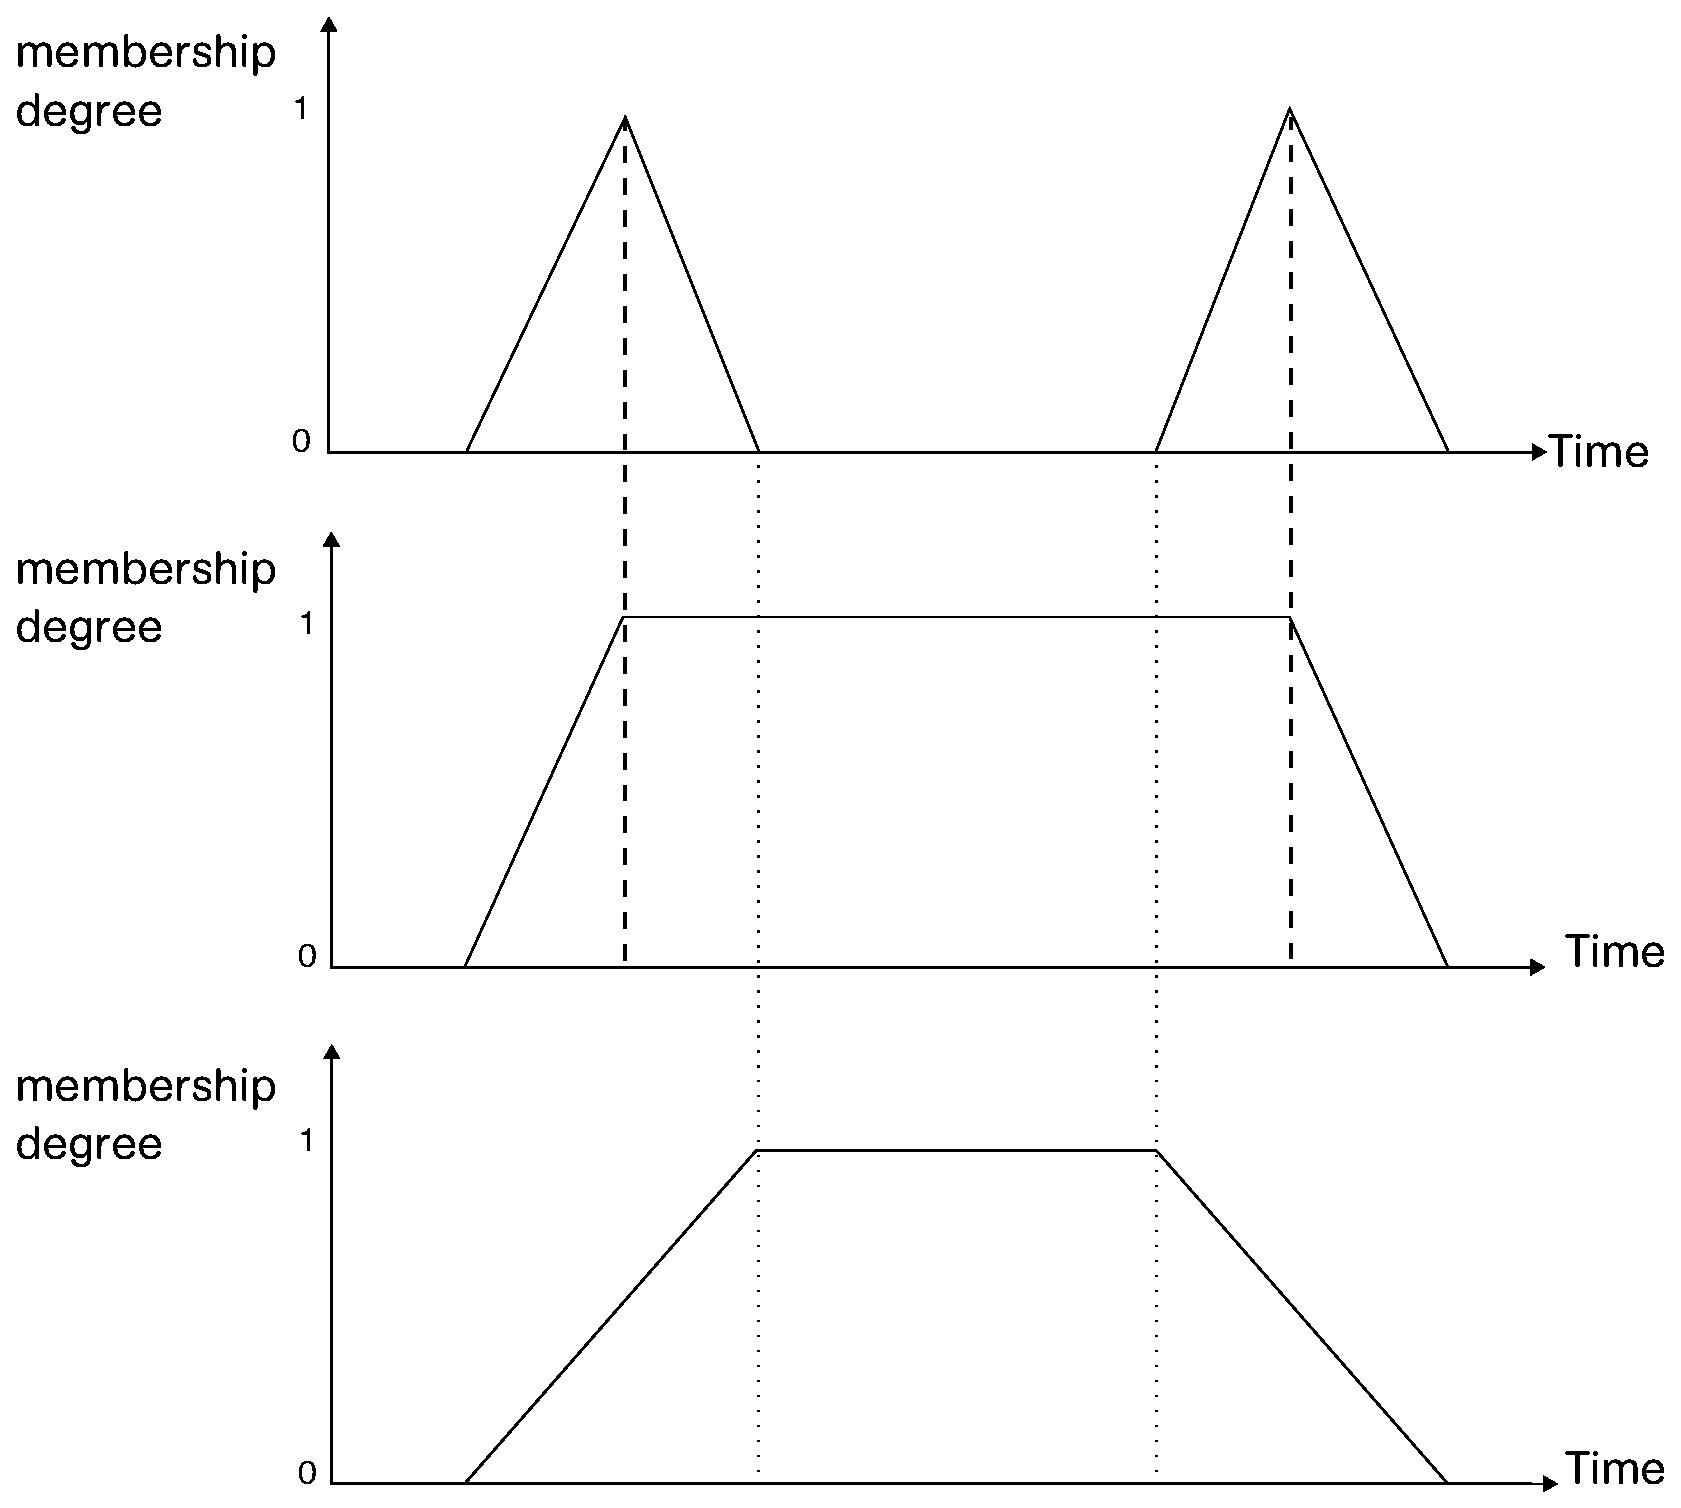
\includegraphics[scale=0.3]{graphs/trapezoidalDistribution.eps}
  \caption{Transformation to obtain the FVP. The top graph shows the two triangular possibility distributions. The middle graph shows the convex hull validity period, the bottom one shows the result of the second transformation, which maintains the imprecision.}
  \label{fig:fuzzy-validity-period}
\end{figure}
%%%%%%%%%%%%%%%%%%%%%%%%%%%%%%
% FVP
%%%%%%%%%%%%%%%%%%%%%%%%%%%%%%%



%
\section{\label{sec:prop}Proposal}
%
%% Proposal
%
%
The model deals with uncertainty in the valid time. A valid time period  \emph{VT} is specified with two points: a starting time point \emph{St} and an ending time point \emph{Et}. Thus, a fuzzy validity period, \emph{FVP} is a valid time period in which the starting, the ending or both points are not precisely known. More formally we make the following definitions:

\begin{definition}
Valid Time Period: bien
\end{definition}

\subsection{Representation}

\subsubsection{Undelying domain: Julian Day Number}

\subsubsection{Temporal Operators}

\subsection{Data Manipulation Language}




\subsection{Query specification}

\begin{example}

\end{example}

%
\section{\label{sec:conc}Conclusions}
%
%We presented a Valid-time model to represent and query ill-known temporal intervals. The main advantage of this framework is that it is always possible to get both a possibility and a necessity measures for every comparison, which is also useful for ranking purposes. The framework models the Allen's relations and it has the flexibility to model specific and more complex relations by means of ill-known constraints.  As future work, the time interval in the query specification would also be ill-known.
%
\subsubsection{Acknowledgements}
%
%%%%%%%%%%%%%%%%%%%%%%%%%%%%%%%%%%%%%%%%%%%%%%%%%%%%%%%%%%%%%%%%%%%%%%%%%
%
% Acknowledgements
%
%%%%%%%%%%%%%%%%%%%%%%%%%%%%%%%%%%%%%%%%%%%%%%%%%%%%%%%%%%%%%%%%%%%%%%%%%
Part of the research is supported by the grant BES-2009-013805 within the research project TIN2008-02066: \emph{Fuzzy Temporal Information treatment in relational DBMS}.



\bibliographystyle{splncs03}
\bibliography{fqas}




\end{document}


